\documentclass[a4paper,11pt]{scrartcl}

\usepackage[ngerman]{babel}
\usepackage[hidelinks]{hyperref}
\usepackage{apacite}
\usepackage{longtable}
\usepackage{tabularx}
\usepackage{gensymb}
\usepackage{amsmath}
\usepackage{graphicx}
\usepackage[left=2cm,right=2cm]{geometry}

\usepackage{fontspec}
    \setmainfont{EB Garamond}
    \setsansfont{Open Sans}
    \setmonofont{DejaVu Sans Mono}

\setcounter{secnumdepth}{0}
\renewcommand{\baselinestretch}{1.2}

\begin{document}

\author{PREN Gruppe 7}
\title{Anforderungsliste}
\date{\today}

\maketitle

\section*{Versionierung}

\def\arraystretch{1.2}
\begin{tabularx}{\textwidth}{|r|l|X|}
\hline
\textsc{Version} & \textsc{Datum} & \textsc{Bemerkung} \\
\hline
0.1 & Do, 05.10.2017 & Zusammentragung sämtlicher Anforderungen \\
0.2 & Di, 10.10.2017 & Dokument zur Vorab-Version für Abgabe vorbereitet; Diskussionsgrundlage für Besprechung am 12. Oktober 2017 \\
0.3 & Do, 12.10.2017 & Anforderungen gemäss Besprechung ergänzt und angepasst \\
1.0 & Fr, 13.10.2017 & Dokument zur Abgabe von Testat 1 vorbereitet \\
1.1 & Do, 14.12.2017 & Kleinere Anpassungen zur Abgabe von Testat 2 durchgeführt \\
1.2 & Di, 09.01.2018 & Finale Überarbeitung gemäss Feedback \\
\hline
\end{tabularx}

\newpage

\section{Anforderungen}

\renewcommand*{\arraystretch}{1.2}
\begin{longtable}{|r|l|l|p{7cm}|l|}
\hline
\textsc{Nr.} & \textsc{Bezeichnung} & \textsc{Stufe\footnote{F: Festanforderung, M: Mindestanforderung, W: Wunsch}} & \textsc{Details} & \textsc{Bereich\footnote{M: Maschinenbau, E: Elektrotechnik, I: Informatik, A: Alle}} \\
\hline
\textsc{1} & \textsc{Rahmenbedingungen}  & & & \\
1.1 & Aufbau & M & \textit{Silisloth} lässt sich in max. zwei Minuten aufbauen. & M \\
1.2 & Autonomie & F & \textit{Silisloth} und das I/O-Gerät arbeiten nach dem Startsignal autonom. & I \\
1.3 & Temperaturbereich & F & Die Komponenten sind in einem Temperaturfenster von $0\degree C$ bis $70\degree C$ einsatzfähig. & M, E, I \\
1.4 & Lichtverhältnisse & F & \textit{Silisloth} funktioniert bei $1’000-100’000$ lux.\footnote{Schwache Beleuchtung bis direkte, starke Sonneneinstrahlung} & E, I \\
1.5 & Zeitrahmen & M & \textit{Silisloth} erledigt ihre Aufgaben innerhalb von vier Minuten. & M, E, I \\
\textsc{2} & \textsc{Dimensionen} & & & \\
2.1 & Länge & M & Max. $480mm$ & M \\
2.2 & Breite & M & Max. $480mm$ & M \\
2.3 & Höhe & M & Max. $580mm$ & M \\
2.4 & Gewicht & M & Max. $7’000g$ Leergewicht von \textit{Silisloth} & M, E, I \\
2.4.1 & & W & Max. $4’000g$ Leergewicht von \textit{Silisloth} & M, E, I \\
\textsc{3} & \textsc{Antrieb} & & & \\
3.1 & Höhenüberwindung & M & \textit{Silisloth} ist in der Lage eine Steigung von max. $40\degree$ zu überwinden. & M \\
3.2 & Einsatzbereich & F & \textit{Silisloth} kann auf einem Seil mit Durchmesser $2-4mm$ montiert werden. & M \\
3.3 & Ziel & F & \textit{Silisloth} stoppt nach Berührung des Endpfostens. & E, I \\
3.4 & Geschwindigkeit & M & \textit{Silisloth} bewegt sich durchschnittlich mit mindestens $15mm/s$.\footnote{4 Minuten Gesamtzeit, ca. $3$ Minuten reine Fahrzeit (ohne Lastaufnahme und Absetzen) für $3.5$ Meter Seil} & E, I, M \\
3.4.1 & & W & \textit{Silisloth} bewegt sich durchschnittlich mit $20mm/s$.\footnote{Die Fahrzeit beträgt dann nur noch 2 Minuten.} & E, I \\
3.5 & Fahrtrichtung & M & \textit{Silisloth} ist in der Lage sich vorwärts und rückwärts am Seil zu bewegen. & M, E, I \\
\textsc{4} & \textsc{Lastbeförderung} & & & \\
4.1 & Greifen & M & \textit{Silisloth} kann eine quaderförmige Last mit den Kantenlängen von mindestens $45mm$ und höchstens $55mm$ und einem Gewicht von bis zu $200g$ greifen.\footnote{Dimension: $(45..55)^{3}mm^{3}=(91'125..166'375)mm^{3}$; spezifisches Gewicht von max. $800kg/m^{3}$ (Buche) = max. ca. $130g$ + Haken $\approx 150g$} & M, E \\
4.2 & Heben/Senken & M & \textit{Silisloth} kann eine Last von bis zu $200g$ heben und senken. & M, E \\
4.3 & Abladen & F & \textit{Silisloth} kann die Last auf dem Zielfeld absetzen. (Genauigkeit: siehe Punkt 5.3 und Unterpunkte) & M, E, I \\
\textsc{5} & \textsc{Sensorik} & & &  \\
5.1 & x-Koordinate & M & Die x-Koordinate muss mit einer Toleranz von $\pm20mm$ bestimmt werden können. & E \\
5.1.1 & & W & Die x-Koordinate muss mit einer Toleranz von $\pm10mm$ bestimmt werden können. & E \\
5.2 & z-Koordinate & M & Die z-Koordinate muss mit einer Toleranz von $\pm20mm$ bestimmt werden können. & E \\
5.2.1 & & W & Die z-Koordinate muss mit einer Toleranz von $\pm10mm$ bestimmt werden können. & E \\
5.3 & Zielerkennung & M & Das spezifizierte Zielfeld muss mit einer Toleranz von $\pm20mm$ erkannt werden können. & E, I \\
5.3.1 & & W & Das spezifizierte Zielfeld muss mit einer Toleranz von $\pm10mm$ erkannt werden können. & E, I \\
5.3.2 & & W & Das Ziel kann während der Fahrt erkannt werden. & E, I \\
5.4 & Lasterkennung & M & Die Last muss mit einer Toleranz von $\pm$15mm erkannt werden können. & E, I \\
5.4.1 & & W & Die Last kann während der Fahrt erkannt werden. & E, I \\
\textsc{6} & \textsc{Kommunikation} & & & \\
6.1 & Startsignal & F & \textit{Silisloth} empfängt das Startsignal. & I \\
6.2 & Koordinaten & F & \textit{Silisloth} sendet die Koordinaten an das Ausgabegerät. & I \\
\textsc{7} & \textsc{I/O-Gerät} & & & \\
7.1 & Startsignal & F & Das Gerät sendet beim Start das Signal an \textit{Silisloth}. & I \\
7.2 & Koordinaten & F & Das Gerät gibt die x- und z-Koordinaten der Last an. & I \\
\textsc{8} & \textsc{Ausnahmebehandlung} & & & \\
8.1 & Masterkennung & F & Falls \textit{Silisloth} den Zielmast nicht erkennt, soll es durch einen Nothalt beim Berühren des Mastes anhalten. & E, I \\
8.2 & Lasterkennung & F & Falls \textit{Silisloth} die Last nicht erkennt, fährt es automatisch zum Ziel. & E, I \\
8.3 & Zielerkennung & F & \textit{Silisloth} lässt die Last beim Zielmast fallen, falls es das Zielfeld nicht erkennt. & E, I \\
8.4 & Schwingen & F & \textit{Silisloth} hält an, falls die Schwingung in y-Richtung $20\degree$ überschreitet & M, E, I \\
8.5 & Lastverlust & F & \textit{Silisloth} erkennt, wenn es die Last verliert. & E, I \\
\hline
\end{longtable}

\begin{figure}
    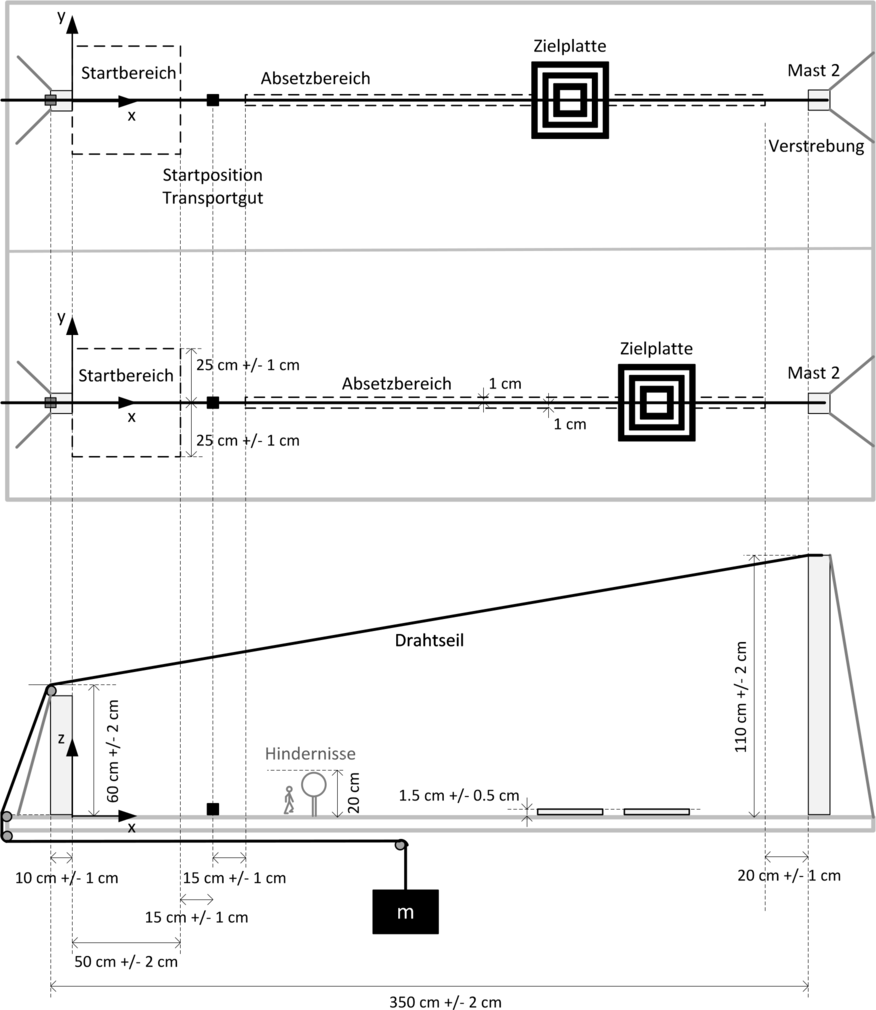
\includegraphics[width=\textwidth]{schema-plattform.png}
    \caption{Plattform, Draufsicht und Seitenansicht, nicht massstäblich (Grafik aus der Aufgabenstellung)}
\end{figure}

\end{document}
